\documentclass[notes,11pt, aspectratio=169]{beamer}

\usepackage{pgfpages}
\setbeameroption{hide notes} % Only slide

\usepackage{array}
\usepackage{tikz}
\usepackage{verbatim}
\setbeamertemplate{note page}{\pagecolor{gray!5}\insertnote}
\usetikzlibrary{positioning}
\usetikzlibrary{snakes}
\usetikzlibrary{calc}
\usetikzlibrary{arrows}
\usetikzlibrary{decorations.markings}
\usetikzlibrary{shapes.misc}
\usetikzlibrary{matrix,shapes,arrows,fit,tikzmark}
\usepackage{amsmath}
\usepackage{mathpazo}
\usepackage{hyperref}
\usepackage{lipsum}
\usepackage{multimedia}
\usepackage{graphicx}
\usepackage{multirow}
\usepackage{dcolumn}
\usepackage{bbm}
\newcolumntype{d}[0]{D{.}{.}{5}}

\usepackage{changepage}
\usepackage{appendixnumberbeamer}

\usepackage[space]{grffile}
\usepackage{booktabs}

% Colors
\definecolor{blue}{RGB}{0,114,178}
\definecolor{red}{RGB}{213,94,0}
\definecolor{yellow}{RGB}{240,228,66}
\definecolor{green}{RGB}{0,158,115}
\definecolor{solutionbg}{RGB}{240,248,240}
\definecolor{solutionframe}{RGB}{0,158,115}

% Solution box environment for worked answers
\usepackage{tcolorbox}
\newtcolorbox{solutionbox}[1][]{
  enhanced,
  colback=solutionbg,
  colframe=solutionframe,
  boxrule=0pt,
  leftrule=3pt,
  arc=0pt,
  left=8pt,
  right=8pt,
  top=6pt,
  bottom=6pt,
  fonttitle=\bfseries,
  title={#1},
  attach boxed title to top left={yshift=-2mm, xshift=5mm},
  boxed title style={colback=solutionframe, colframe=solutionframe, size=small, arc=2pt}
}

\hypersetup{
  colorlinks=false,
  linkbordercolor = {white},
  linkcolor = {blue}
}

\definecolor{MyBackground}{RGB}{255,253,218}

\newenvironment{transitionframe}{
  \setbeamercolor{background canvas}{bg=white}
  \begin{frame}}{
    \end{frame}
}

\setbeamercolor{frametitle}{fg=blue}
\setbeamercolor{title}{fg=black}
\setbeamertemplate{footline}[frame number]
\setbeamertemplate{navigation symbols}{}
\setbeamertemplate{itemize items}{-}
\setbeamercolor{itemize item}{fg=blue}
\setbeamercolor{itemize subitem}{fg=blue}
\setbeamercolor{enumerate item}{fg=blue}
\setbeamercolor{enumerate subitem}{fg=blue}
\setbeamercolor{button}{bg=MyBackground,fg=blue,}

\setbeamercolor{section in toc}{fg=blue}
\setbeamercolor{subsection in toc}{fg=red}
\setbeamersize{text margin left=1em,text margin right=1em}

\newenvironment{wideitemize}{\itemize\addtolength{\itemsep}{10pt}}{\enditemize}
\newenvironment{wideenumerate}{\enumerate\addtolength{\itemsep}{10pt}}{\endenumerate}

\title[]{\textcolor{blue}{ECN 594: Two-Part Tariffs and Self-Selection}}
\author[PGP]{}
\institute[FRBNY]{\small{\begin{tabular}{c c c}
Nicholas Vreugdenhil \\
\end{tabular}}}
\date{\today}

\begin{document}

% Title Slide
\begin{frame}
\maketitle
  \centering
\end{frame}

\begin{frame}{Plan}
  \begin{wideenumerate}
    \item \textbf{Two-part tariffs: structure and intuition}
    \item Optimal two-part tariff (homogeneous consumers)
    \item Heterogeneous consumers (brief)
    \item[] \rule{0.5\textwidth}{0.4pt}
    \item Self-selection: versioning and menu design
    \item Incentive compatibility and individual rationality
    \item Worked example: optimal menu
  \end{wideenumerate}
\end{frame}

%%%%%%%%%%%%%%%%%%%%%%%%%%%%%%%%%%%%%%%%%%%%%%%%%%%%%%%%%%%%%
% TWO-PART TARIFFS
%%%%%%%%%%%%%%%%%%%%%%%%%%%%%%%%%%%%%%%%%%%%%%%%%%%%%%%%%%%%%

\begin{frame}{Plan}
  \begin{wideenumerate}
    \item \textbf{Two-part tariffs: structure and intuition}
    \item Optimal two-part tariff (homogeneous consumers)
    \item Heterogeneous consumers (brief)
    \item[] \rule{0.5\textwidth}{0.4pt}
    \item Self-selection: versioning and menu design
    \item Incentive compatibility and individual rationality
    \item Worked example: optimal menu
  \end{wideenumerate}
\end{frame}

\begin{frame}{Non-linear pricing}
	\begin{wideitemize}
		\item So far: price discrimination by \textbf{selection by indicators}
		\begin{wideitemize}
			\vspace{5pt}
			\item Requires observable characteristics (student ID, location, etc.)
		\end{wideitemize}
		\item Now: \textbf{non-linear pricing}
		\begin{wideitemize}
			\vspace{5pt}
			\item Price per unit depends on quantity purchased
			\item Consumers \textit{self-select} into how much to buy
		\end{wideitemize}
		\item Key example: \textbf{two-part tariffs}
	\end{wideitemize}
\end{frame}

\begin{frame}{Two-part tariff structure}
	\begin{wideitemize}
		\item A two-part tariff has the form:
		\begin{align*}
			\text{Total payment} = F + p \times q
		\end{align*}
		\item $F$: fixed fee (membership, connection charge)
		\item $p$: per-unit price (price per unit consumed)
		\item $q$: quantity consumed
		\item \textbf{Examples:}
		\begin{wideitemize}
			\vspace{5pt}
			\item Golf club: membership fee + greens fee per round
			\item Phone plan: monthly fee + per-minute charges
			\item Costco: annual membership + price per item
		\end{wideitemize}
	\end{wideitemize}
\end{frame}

\begin{frame}{Worked example: Gym membership}
	\begin{wideitemize}
		\item \textbf{Question:}
		\item A gym knows each member has demand $q = 20 - 2p$ (visits per month).
		\item $MC = 2$ per visit.
		\item What is the optimal two-part tariff ($F$, $p$)?
		\item How much profit per member?
	\end{wideitemize}
	\vspace{15pt}
	\centering
	\textit{Take 3 minutes to solve this.}
\end{frame}

\begin{frame}{Worked example: Gym membership (solution)}
	\begin{solutionbox}[Solution]
		\begin{wideitemize}
			\item \textbf{Step 1:} Set $p = MC = 2$
			\item At $p = 2$: $q = 20 - 2(2) = 16$ visits
			\item \textbf{Step 2:} Compute CS at $p = 2$
			\begin{wideitemize}
				\vspace{3pt}
				\item Max WTP (intercept): $p = 10$ when $q = 0$
				\item $CS = \frac{1}{2} \times 16 \times (10 - 2) = \frac{1}{2} \times 16 \times 8 = 64$
			\end{wideitemize}
			\item \textbf{Step 3:} Set $F = CS = 64$
			\item \textbf{Optimal tariff:} \$64/month + \$2/visit
			\item \textbf{Profit per member:} \$64 (all from the fixed fee!)
		\end{wideitemize}
	\end{solutionbox}
\end{frame}

\begin{frame}{Why is this ``non-linear''?}
	\begin{wideitemize}
		\item Average price per unit: $\frac{F + pq}{q} = p + \frac{F}{q}$
		\item As $q$ increases, average price \textbf{decreases}
		\item This is a quantity discount!
		\item The pricing is ``non-linear'' because total payment is not proportional to quantity
	\end{wideitemize}
\end{frame}

\begin{frame}{Plan}
  \begin{wideenumerate}
    \item Two-part tariffs: structure and intuition
    \item \textbf{Optimal two-part tariff (homogeneous consumers)}
    \item Heterogeneous consumers (brief)
    \item[] \rule{0.5\textwidth}{0.4pt}
    \item Self-selection: versioning and menu design
    \item Incentive compatibility and individual rationality
    \item Worked example: optimal menu
  \end{wideenumerate}
\end{frame}

\begin{frame}{Why use two-part tariffs?}
	\begin{columns}
		\begin{column}{0.5\textwidth}
			\begin{figure}
				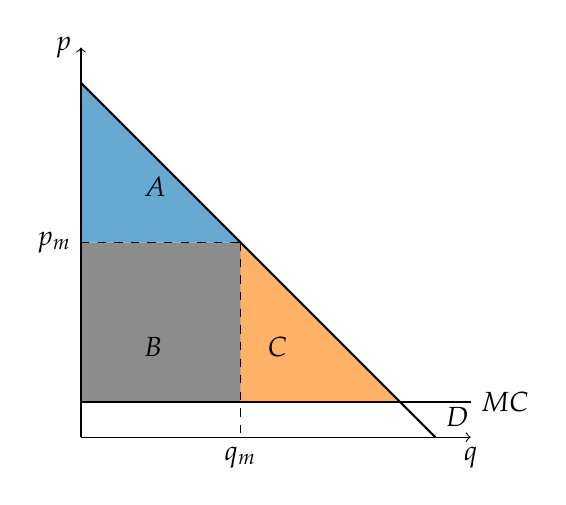
\begin{tikzpicture}[scale=0.45]
					\fill [darkgray!60] (0,1) -- (0,5.5) -- (4.5,5.5) -- (5.5,1) -- cycle;
					\fill [blue!60] (0,5.5) -- (4.5,5.5) -- (0,10) -- cycle;
					\fill [orange!60] (4.5,1) -- (4.5,5.5) -- (9,1) -- cycle;

					\draw [->] (0,0) to (0,11) node [left] {$p$};
					\draw [->] (0,0) to (11,0) node [below] {$q$};
					\draw [thick] (0,10)  to  (10,0)  node [above right] {$D$};
					\draw [thick] (0,1)  to  (11,1)  node [right] {$MC$};

					\draw [dashed] (0,5.5) node [left] {$p_m$} to (4.55,5.5);
					\draw [dashed] (4.5,5.5) to (4.5,0) node [below] {$q_m$};

					\node [above right] at (1.5,6.5) {$A$};
					\node [above right] at (5,2) {$C$};
					\node [above right] at (1.5,2) {$B$};
				\end{tikzpicture}
			\end{figure}
		\end{column}
		\begin{column}{0.5\textwidth}
			\begin{wideitemize}
				\item Under uniform pricing at $p_m$:
				\begin{wideitemize}
					\vspace{5pt}
					\item CS = Area $A$
					\item Profit = Area $B$
					\item DWL = Area $C$
				\end{wideitemize}
				\item Monopolist ``leaves money on the table''
				\item Can we do better?
			\end{wideitemize}
		\end{column}
	\end{columns}
\end{frame}

\begin{frame}{Optimal two-part tariff: homogeneous consumers}
	\begin{wideitemize}
		\item Assume all consumers are identical (same demand curve)
		\item \textbf{Key insight:} Use $F$ to extract surplus, use $p$ to maximize total surplus
		\item \textbf{Step 1:} Set $p = MC$
		\begin{wideitemize}
			\vspace{5pt}
			\item This maximizes total surplus (eliminates DWL)
		\end{wideitemize}
		\item \textbf{Step 2:} Set $F = CS(p = MC)$
		\begin{wideitemize}
			\vspace{5pt}
			\item Extract all consumer surplus through the fixed fee
		\end{wideitemize}
	\end{wideitemize}
\end{frame}

\begin{frame}{Optimal two-part tariff: graphically}
	\begin{columns}
		\begin{column}{0.5\textwidth}
			\begin{figure}
				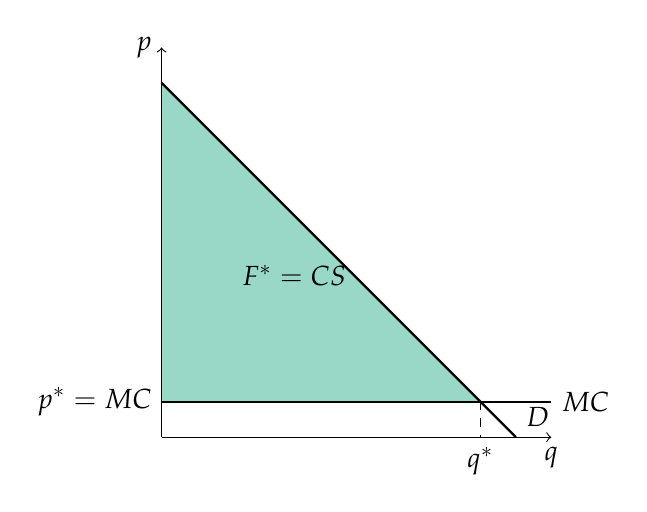
\begin{tikzpicture}[scale=0.45]
					\fill [green!40] (0,1) -- (0,10) -- (9,1) -- cycle;

					\draw [->] (0,0) to (0,11) node [left] {$p$};
					\draw [->] (0,0) to (11,0) node [below] {$q$};
					\draw [thick] (0,10)  to  (10,0)  node [above right] {$D$};
					\draw [thick] (0,1)  to  (11,1)  node [right] {$MC$};

					\draw [dashed] (9,1) to (9,0) node [below] {$q^*$};

					\node [above right] at (2,4) {$F^* = CS$};
					\node [left] at (0,1) {$p^*=MC$};
				\end{tikzpicture}
			\end{figure}
		\end{column}
		\begin{column}{0.5\textwidth}
			\begin{wideitemize}
				\item Set $p^* = MC$
				\item Consumers buy $q^*$ (efficient quantity)
				\item Set $F^* = $ entire green triangle
				\item Profit = $F^* - 0 = F^*$
				\item \textbf{Result:} Firm captures ALL surplus
			\end{wideitemize}
		\end{column}
	\end{columns}
\end{frame}

\begin{frame}{Worked example: Two-part tariff}
	\begin{wideitemize}
		\item \textbf{Question:} Individual demand is $q = 15 - 2.5p$. Marginal cost is $MC = 0$.
		\item (a) What is the optimal uniform price and profit per consumer?
		\item (b) What is the optimal two-part tariff and profit per consumer?
	\end{wideitemize}
	\vspace{15pt}
	\centering
	\textit{Take 5 minutes to solve this.}
\end{frame}

\begin{frame}{Worked example: Two-part tariff (solution)}
	\begin{solutionbox}[Solution]
		\begin{wideitemize}
			\item \textbf{(a) Uniform pricing:}
			\begin{wideitemize}
				\vspace{3pt}
				\item Inverse demand: $p = 6 - q/2.5$
				\item $MR = 6 - 2q/2.5 = 6 - 0.8q$
				\item Set $MR = MC$: $6 - 0.8q = 0 \Rightarrow q = 7.5$
				\item Price: $p = 6 - 7.5/2.5 = 3$
				\item Profit: $\pi = 3 \times 7.5 = 22.5$ per consumer
			\end{wideitemize}
			\item \textbf{(b) Two-part tariff:}
			\begin{wideitemize}
				\vspace{3pt}
				\item Set $p = MC = 0$
				\item At $p = 0$: $q = 15$
				\item $CS = \frac{1}{2} \times 15 \times 6 = 45$
				\item Set $F = 45$
				\item Profit: $\pi = 45$ per consumer (double the uniform price!)
			\end{wideitemize}
		\end{wideitemize}
	\end{solutionbox}
\end{frame}

\begin{frame}{Welfare effects of two-part tariffs}
	\begin{wideitemize}
		\item Compared to uniform monopoly pricing:
		\item \textbf{Producer surplus:} Increases (captures all surplus)
		\item \textbf{Consumer surplus:} Decreases to zero
		\item \textbf{Total surplus:} Increases (DWL eliminated!)
		\item \textbf{Efficiency vs equity tradeoff:}
		\begin{wideitemize}
			\vspace{5pt}
			\item More efficient (no DWL)
			\item Less equitable (consumers get nothing)
		\end{wideitemize}
	\end{wideitemize}
\end{frame}

\begin{frame}{Plan}
  \begin{wideenumerate}
    \item Two-part tariffs: structure and intuition
    \item Optimal two-part tariff (homogeneous consumers)
    \item \textbf{Heterogeneous consumers (brief)}
    \item[] \rule{0.5\textwidth}{0.4pt}
    \item Self-selection: versioning and menu design
    \item Incentive compatibility and individual rationality
    \item Worked example: optimal menu
  \end{wideenumerate}
\end{frame}

\begin{frame}{What about heterogeneous consumers?}
	\begin{wideitemize}
		\item Reality: consumers have different demand curves
		\item Problem: if $F$ is too high, some consumers don't participate
		\item \textbf{Tradeoff:}
		\begin{wideitemize}
			\vspace{5pt}
			\item High $F$: extract more from high-value consumers, but lose low-value ones
			\item Low $F$: serve more consumers, but extract less per consumer
		\end{wideitemize}
		\item Optimal $F$ balances these effects
		\item Often: $p > MC$ (to extract more from high-demand consumers through variable pricing)
	\end{wideitemize}
\end{frame}

\begin{frame}{Worked example: Two-part tariff with two types}
	\begin{wideitemize}
		\item \textbf{Question:}
		\item Type H: demand $q_H = 10 - p$, 100 consumers
		\item Type L: demand $q_L = 5 - p$, 200 consumers
		\item $MC = 0$
		\item Compare: (a) $F = 50, p = 0$ vs (b) $F = 12.5, p = 0$
	\end{wideitemize}
	\vspace{15pt}
	\centering
	\textit{Take 3 minutes to solve this.}
\end{frame}

\begin{frame}{Worked example: Two-part tariff with two types (solution)}
	\begin{solutionbox}[Solution]
		\begin{wideitemize}
			\item \textbf{(a) $F = 50, p = 0$:}
			\begin{wideitemize}
				\vspace{3pt}
				\item Type H: $CS = \frac{1}{2}(10)(10) = 50 \geq F$ $\checkmark$ joins
				\item Type L: $CS = \frac{1}{2}(5)(5) = 12.5 < F$ doesn't join
				\item Profit $= 50 \times 100 = \$5,000$
			\end{wideitemize}
			\item \textbf{(b) $F = 12.5, p = 0$:}
			\begin{wideitemize}
				\vspace{3pt}
				\item Type H: $CS = 50 \geq 12.5$ $\checkmark$ joins
				\item Type L: $CS = 12.5 \geq 12.5$ $\checkmark$ joins
				\item Profit $= 12.5 \times 300 = \$3,750$
			\end{wideitemize}
			\item \textbf{Better to serve only H!} (in this case)
		\end{wideitemize}
	\end{solutionbox}
\end{frame}

%%%%%%%%%%%%%%%%%%%%%%%%%%%%%%%%%%%%%%%%%%%%%%%%%%%%%%%%%%%%%
% SELF-SELECTION
%%%%%%%%%%%%%%%%%%%%%%%%%%%%%%%%%%%%%%%%%%%%%%%%%%%%%%%%%%%%%

\begin{frame}{Plan}
  \begin{wideenumerate}
    \item Two-part tariffs: structure and intuition
    \item Optimal two-part tariff (homogeneous consumers)
    \item Heterogeneous consumers (brief)
    \item[] \rule{0.5\textwidth}{0.4pt}
    \item \textbf{Self-selection: versioning and menu design}
    \item Incentive compatibility and individual rationality
    \item Worked example: optimal menu
  \end{wideenumerate}
\end{frame}

\begin{frame}{The self-selection problem: why can't we just ask?}
	\begin{wideitemize}
		\item \textbf{Why not ask consumers their WTP directly?}
		\item Everyone would claim to be a low-value buyer!
		\item \textbf{Information asymmetry:}
		\begin{wideitemize}
			\vspace{5pt}
			\item Consumers know their type
			\item Firm does not
			\item Consumers have incentive to misreport
		\end{wideitemize}
		\item \textbf{Solution:} Design options so that revealing type is in consumers' interest
	\end{wideitemize}
\end{frame}

\begin{frame}{Self-selection: the idea}
	\begin{wideitemize}
		\item \textbf{Problem:} Seller cannot directly observe consumer types
		\begin{wideitemize}
			\vspace{5pt}
			\item Can't tell who has high vs low willingness to pay
		\end{wideitemize}
		\item \textbf{Solution:} Design a \textbf{menu} of options
		\begin{wideitemize}
			\vspace{5pt}
			\item Different options appeal to different types
			\item Consumers ``self-select'' into revealing their type
		\end{wideitemize}
		\item Also called: screening, menu design, second-degree price discrimination
	\end{wideitemize}
\end{frame}

\begin{frame}{Self-selection: versioning}
	\begin{wideitemize}
		\item \textbf{Versioning:} Offer different ``versions'' of a product
		\begin{wideitemize}
			\vspace{5pt}
			\item High-quality version for high-value consumers
			\item Low-quality version for low-value consumers
		\end{wideitemize}
		\item \textbf{Examples:}
		\begin{wideitemize}
			\vspace{5pt}
			\item Airline tickets: business class vs economy
			\item Software: Pro vs Basic editions
			\item iPhone Pro vs iPhone
		\end{wideitemize}
		\item \textbf{Damaged goods:} Sometimes firms deliberately reduce quality
		\begin{wideitemize}
			\vspace{5pt}
			\item Tesla: software-limited battery range
			\item 19th century French rail: roofless third-class cars
		\end{wideitemize}
	\end{wideitemize}
\end{frame}

\begin{frame}{The menu design problem: setup}
	\begin{wideitemize}
		\item Two consumer types: H (high-value) and L (low-value)
		\item Two product versions: Full and Stripped-down
		\item Willingness to pay:
		\begin{center}
			\begin{tabular}{|c|c|c|}
				\hline
				& Full & Stripped-down \\
				\hline
				Type H & $v_H^F$ & $v_H^S$ \\
				Type L & $v_L^F$ & $v_L^S$ \\
				\hline
			\end{tabular}
		\end{center}
		\item Assume: $v_H^F > v_L^F$ and $v_H^S > v_L^S$ (H values both more)
		\item Also: $v_H^F - v_H^S > v_L^F - v_L^S$ (H values upgrade more)
	\end{wideitemize}
\end{frame}

\begin{frame}{Consumer choice: self-selection}
	\begin{wideitemize}
		\item Consumer surplus from each option:
		\begin{align*}
			CS_{\text{Full}} &= v^F - p_F \\
			CS_{\text{Stripped}} &= v^S - p_S
		\end{align*}
		\item Each consumer chooses the option with highest CS
		\item (If both negative, consumer doesn't buy)
	\end{wideitemize}
\end{frame}

\begin{frame}{Plan}
  \begin{wideenumerate}
    \item Two-part tariffs: structure and intuition
    \item Optimal two-part tariff (homogeneous consumers)
    \item Heterogeneous consumers (brief)
    \item[] \rule{0.5\textwidth}{0.4pt}
    \item Self-selection: versioning and menu design
    \item \textbf{Incentive compatibility and individual rationality}
    \item Worked example: optimal menu
  \end{wideenumerate}
\end{frame}

\begin{frame}{Constraints on pricing}
	\begin{wideitemize}
		\item \textbf{Incentive Compatibility (IC):} Each type prefers ``their'' option
		\begin{align*}
			\text{IC}_H: \quad v_H^F - p_F &\geq v_H^S - p_S \\
			\text{IC}_L: \quad v_L^S - p_S &\geq v_L^F - p_F
		\end{align*}
		\item \textbf{Individual Rationality (IR):} Each type is willing to participate
		\begin{align*}
			\text{IR}_H: \quad v_H^F - p_F &\geq 0 \\
			\text{IR}_L: \quad v_L^S - p_S &\geq 0
		\end{align*}
		\item Also called: participation constraints
	\end{wideitemize}
\end{frame}

\begin{frame}{Key insight: which constraints bind?}
	\begin{wideitemize}
		\item In the optimal menu:
		\begin{wideitemize}
			\vspace{5pt}
			\item $\text{IC}_H$ binds: H is just indifferent between Full and Stripped
			\item $\text{IR}_L$ binds: L gets zero surplus from Stripped
		\end{wideitemize}
		\item \textbf{Intuition:}
		\begin{wideitemize}
			\vspace{5pt}
			\item Extract all surplus from L (low type has no ``outside option'')
			\item H gets some surplus (to prevent them from mimicking L)
		\end{wideitemize}
		\item This is called: ``no distortion at the top''
	\end{wideitemize}
\end{frame}

\begin{frame}{Plan}
  \begin{wideenumerate}
    \item Two-part tariffs: structure and intuition
    \item Optimal two-part tariff (homogeneous consumers)
    \item Heterogeneous consumers (brief)
    \item[] \rule{0.5\textwidth}{0.4pt}
    \item Self-selection: versioning and menu design
    \item Incentive compatibility and individual rationality
    \item \textbf{Worked example: optimal menu}
  \end{wideenumerate}
\end{frame}

\begin{frame}{Worked example: Airline pricing}
	\begin{wideitemize}
		\item \textbf{Question:}
		\item Business travelers (B): WTP \$800 for flexible, \$400 for restricted
		\item Leisure travelers (L): WTP \$300 for flexible, \$250 for restricted
		\item 100 of each type. $MC = 100$ for both ticket types.
		\item Design the optimal menu (prices for flexible and restricted).
	\end{wideitemize}
	\vspace{15pt}
	\centering
	\textit{Take 4 minutes to solve this.}
\end{frame}

\begin{frame}{Worked example: Airline pricing (solution)}
	\begin{solutionbox}[Solution]
		\begin{wideitemize}
			\item \textbf{Step 1:} Set $IR_L$ to bind: $p_R = 250$ (L gets zero surplus)
			\item \textbf{Step 2:} Set $IC_B$ to bind:
			\begin{align*}
				800 - p_F &= 400 - 250 \\
				p_F &= 800 - 150 = 650
			\end{align*}
			\item \textbf{Check L doesn't want flexible:} $300 - 650 = -350 < 0$ $\checkmark$
			\item \textbf{Profit:}
			\begin{align*}
				\pi = (650 - 100) \times 100 + (250 - 100) \times 100 = 55,000 + 15,000 = 70,000
			\end{align*}
			\item B gets rent of \$150 (to prevent mimicking L)
		\end{wideitemize}
	\end{solutionbox}
\end{frame}

\begin{frame}{Worked example: Versioning}
	\begin{wideitemize}
		\item Two product versions. $MC = 300$ for both.
		\item 1 million type H consumers; 2 million type L consumers
		\item Willingness to pay:
		\begin{center}
			\begin{tabular}{|c|c|c|}
				\hline
				& Full & Stripped \\
				\hline
				Type H & 1500 & 800 \\
				Type L & 600 & 500 \\
				\hline
			\end{tabular}
		\end{center}
		\item \textbf{Questions:}
		\item (a) Profit from selling only Full at $p_F = 1500$?
		\item (b) Profit from $p_F = 1500$, $p_S = 500$?
		\item (c) Profit from $p_F = 1200$, $p_S = 500$?
	\end{wideitemize}
	\vspace{10pt}
	\centering
	\textit{Take 5 minutes to solve this.}
\end{frame}

\begin{frame}{Worked example: Versioning (solution part a)}
	\begin{solutionbox}[Solution]
		\begin{wideitemize}
			\item \textbf{(a) Only Full at $p_F = 1500$:}
			\begin{wideitemize}
				\vspace{5pt}
				\item Type H: $CS = 1500 - 1500 = 0 \geq 0$ $\checkmark$ (buys)
				\item Type L: $CS = 600 - 1500 = -900 < 0$ (doesn't buy)
			\end{wideitemize}
			\item Only H buys
			\item Profit $= (1500 - 300) \times 1\text{M} = \$1.2\text{B}$
		\end{wideitemize}
	\end{solutionbox}
\end{frame}

\begin{frame}{Worked example: Versioning (solution part b)}
	\begin{solutionbox}[Solution]
		\begin{wideitemize}
			\item \textbf{(b) $p_F = 1500$, $p_S = 500$:}
			\item Type H:
			\begin{wideitemize}
				\vspace{3pt}
				\item $CS_F = 1500 - 1500 = 0$
				\item $CS_S = 800 - 500 = 300$ $\leftarrow$ \textbf{higher!}
			\end{wideitemize}
			\item Type H buys Stripped! (IC violated)
			\item Type L: $CS_S = 500 - 500 = 0$ (buys Stripped)
			\item Everyone buys Stripped
			\item Profit $= (500 - 300) \times 3\text{M} = \$600\text{M}$
			\item \textbf{Worse than (a)!} The menu is poorly designed.
		\end{wideitemize}
	\end{solutionbox}
\end{frame}

\begin{frame}{Worked example: Versioning (solution part c)}
	\begin{solutionbox}[Solution]
		\begin{wideitemize}
			\item \textbf{(c) $p_F = 1200$, $p_S = 500$:}
			\item Type H:
			\begin{wideitemize}
				\vspace{3pt}
				\item $CS_F = 1500 - 1200 = 300$
				\item $CS_S = 800 - 500 = 300$
			\end{wideitemize}
			\item H is indifferent $\rightarrow$ buys Full (IC binds!)
			\item Type L: $CS_F = 600 - 1200 = -600$, $CS_S = 500 - 500 = 0$
			\item L buys Stripped (IR binds!)
			\item Profit $= (1200 - 300) \times 1\text{M} + (500 - 300) \times 2\text{M} = \$1.3\text{B}$
			\item \textbf{Best of the three!}
		\end{wideitemize}
	\end{solutionbox}
\end{frame}

\begin{frame}{Lessons from the example}
	\begin{wideitemize}
		\item The optimal menu satisfies:
		\begin{wideenumerate}
			\vspace{5pt}
			\item IC for H binds: H just willing to buy Full over Stripped
			\item IR for L binds: L gets exactly zero surplus
		\end{wideenumerate}
		\item H gets ``information rent'' (surplus of 300)
		\begin{wideitemize}
			\vspace{5pt}
			\item This is the cost of preventing H from mimicking L
		\end{wideitemize}
		\item Price gap $p_F - p_S$ must be $\leq v_H^F - v_H^S$ (otherwise H switches)
	\end{wideitemize}
\end{frame}

\begin{frame}{Why ``damaged goods''?}
	\begin{wideitemize}
		\item Sometimes the low-quality version costs \textit{more} to produce!
		\item Example: Tesla battery-limited car
		\begin{wideitemize}
			\vspace{5pt}
			\item Same car, same battery, just software restriction
			\item \textbf{Why?} To prevent high-value buyers from choosing the cheap option
		\end{wideitemize}
		\item By making the low-quality version less attractive to H types, the firm can:
		\begin{wideitemize}
			\vspace{5pt}
			\item Charge more for the high-quality version
			\item Still serve the low-value market
		\end{wideitemize}
	\end{wideitemize}
\end{frame}

\begin{frame}{Classic example: Intel 486 processor}
	\begin{wideitemize}
		\item Intel 486DX: full-featured processor
		\item Intel 486SX: same chip, but with math coprocessor \textbf{disabled}
		\item 486SX costs \textbf{more} to produce (extra step to disable!)
		\item \textbf{Why?}
		\begin{wideitemize}
			\vspace{5pt}
			\item Creates price discrimination without observable characteristics
			\item Business users (need math) pay more for 486DX
			\item Home users (don't need math) self-select into 486SX
		\end{wideitemize}
		\item Same logic as Tesla battery restrictions today
	\end{wideitemize}
\end{frame}

\begin{frame}{iPhone storage: versioning in action}
	\begin{wideitemize}
		\item iPhone comes in 128GB, 256GB, 512GB versions
		\item Cost difference to Apple: maybe \$20-30
		\item Price difference to consumers: \$100-200
		\item \textbf{Why such large price gaps?}
		\begin{wideitemize}
			\vspace{5pt}
			\item High-value users (professionals, photographers) need more storage
			\item They're willing to pay much more
			\item Low-value users self-select into smaller storage
		\end{wideitemize}
		\item This is versioning through product attributes
	\end{wideitemize}
\end{frame}

\begin{frame}{Self-selection: cookbook summary}
	\begin{wideenumerate}
		\item Compute consumer surplus for each type, for each option:
		\begin{align*}
			CS = WTP - price
		\end{align*}
		\item For each type, find the option with highest CS
		\item Check that CS $\geq 0$ (otherwise they don't buy)
		\item Compute profit given consumer choices
		\item To find optimal prices: set IC for H and IR for L to bind
	\end{wideenumerate}
\end{frame}

\begin{frame}{Summary: When does each type of price discrimination apply?}
	\begin{center}
	\begin{tabular}{|l|l|l|}
		\hline
		\textbf{Type} & \textbf{Key requirement} & \textbf{Examples} \\
		\hline
		Selection by & Observable & Students, seniors, \\
		indicators & characteristic & geographic regions \\
		\hline
		Two-part & Can charge & Gym, Costco, \\
		tariffs & fixed + variable & phone plans \\
		\hline
		Self-selection & Can offer & Airline classes, \\
		(versioning) & different versions & software editions \\
		\hline
	\end{tabular}
	\end{center}
	\vspace{10pt}
	\begin{wideitemize}
		\item All require: \textbf{market power} and \textbf{inability to resell}
	\end{wideitemize}
\end{frame}

\begin{frame}{Connection to demand estimation}
	\begin{wideitemize}
		\item Demand estimation gives us \textbf{elasticities by consumer type}
		\item This directly informs pricing strategy:
		\begin{wideitemize}
			\vspace{5pt}
			\item \textbf{Selection by indicators:} Different prices for observable groups
			\item \textbf{Versioning:} Design features that appeal differently to types
		\end{wideitemize}
		\item \textbf{Example:} If demand estimation shows:
		\begin{wideitemize}
			\vspace{5pt}
			\item Business travelers inelastic, value flexibility
			\item Leisure travelers elastic, value low price
		\end{wideitemize}
		\item $\Rightarrow$ Offer flexible tickets at high price, restricted at low price
	\end{wideitemize}
\end{frame}

\begin{frame}{Preparing for the midterm}
	\begin{wideitemize}
		\item \textbf{Topics covered so far:}
		\begin{wideenumerate}
			\vspace{5pt}
			\item Demand estimation: logit, Berry inversion, elasticities, IVs
			\item Consumer surplus: log-sum formula
			\item Price discrimination: selection by indicators, two-part tariffs, self-selection
		\end{wideenumerate}
		\item \textbf{Key skills:}
		\begin{wideitemize}
			\vspace{5pt}
			\item Compute elasticities from logit model
			\item Apply Lerner index to find optimal prices
			\item Set up and solve menu design problems with IC/IR constraints
		\end{wideitemize}
		\item Next lecture: Review session with practice problems
	\end{wideitemize}
\end{frame}

%%%%%%%%%%%%%%%%%%%%%%%%%%%%%%%%%%%%%%%%%%%%%%%%%%%%%%%%%%%%%
% KEY POINTS
%%%%%%%%%%%%%%%%%%%%%%%%%%%%%%%%%%%%%%%%%%%%%%%%%%%%%%%%%%%%%

\begin{frame}{Key Points}
	\vspace{11pt}
	\begin{wideenumerate}
		\item \textbf{Two-part tariff:} $F + p \times q$ (fixed fee + per-unit price)
		\item \textbf{Optimal (homogeneous):} Set $p = MC$, $F = CS$ at that price
		\item Two-part tariffs increase efficiency but reduce consumer surplus to zero
		\item \textbf{Self-selection:} Design menu so types reveal themselves
		\item \textbf{IC constraint:} Each type prefers ``their'' option
		\item \textbf{IR constraint:} Each type willing to participate (CS $\geq 0$)
		\item Optimal menu: IC binds for high type, IR binds for low type
		\item High type gets ``information rent''; low type gets zero surplus
	\end{wideenumerate}
\end{frame}

\begin{frame}{Next time}
	\begin{wideitemize}
		\item \textbf{Lecture 6:} Review for Midterm
		\begin{wideitemize}
			\vspace{5pt}
			\item Demand estimation: logit, Berry inversion, IVs
			\item Pricing: monopoly, price discrimination, two-part tariffs
			\item Practice problems
		\end{wideitemize}
		\item \textbf{HW1 due before Lecture 6}
	\end{wideitemize}
\end{frame}

\end{document}
